\chapter{Planning}
\label{chap:planning}

Pour faire le planning, j'ai décidé de l'intégrer le plus possible à Gitlab. En effet, j'ai choisi d'utiliser les épics, les issues et les milestones disponibles directement sur Gitlab.
Les avantages sont que le planing est très bien intégré et qu'on peut récupérer l'historique précis des actions effectuées pour compléter la tâche.
En revanche, le diagramme de Gantt n'est pas pratique à utiliser et le point de vue est orienté sur les tâches et non sur le timing.

Pour organiser le travail, j'ai choisi d'utiliser deux niveaux d'épics. Le premier représente les objectifs principaux, ceux-ci sont complétés par des sous épics qui sont les tâches à effectuer.
Ce deuxième niveau est complété par des issues qui sont les étapes à cocher pour compléter une tâche. Sur ces issues, on indiquera le poids afin de pouvoir quantifier l'effort nécessaire à la réalisation et on pourra lier des merge requests pour garder une trace des modifications.
Les milestones sont là pour rappeler les échances de différents rendus.

Le planning est directement accessible dans le menu "Roadmap" du groupe Gitlab (\href{https://gitlab.forge.hefr.ch/groups/ps5-2223-fusionprediction/-/roadmap}{lien}).

\begin{center}
    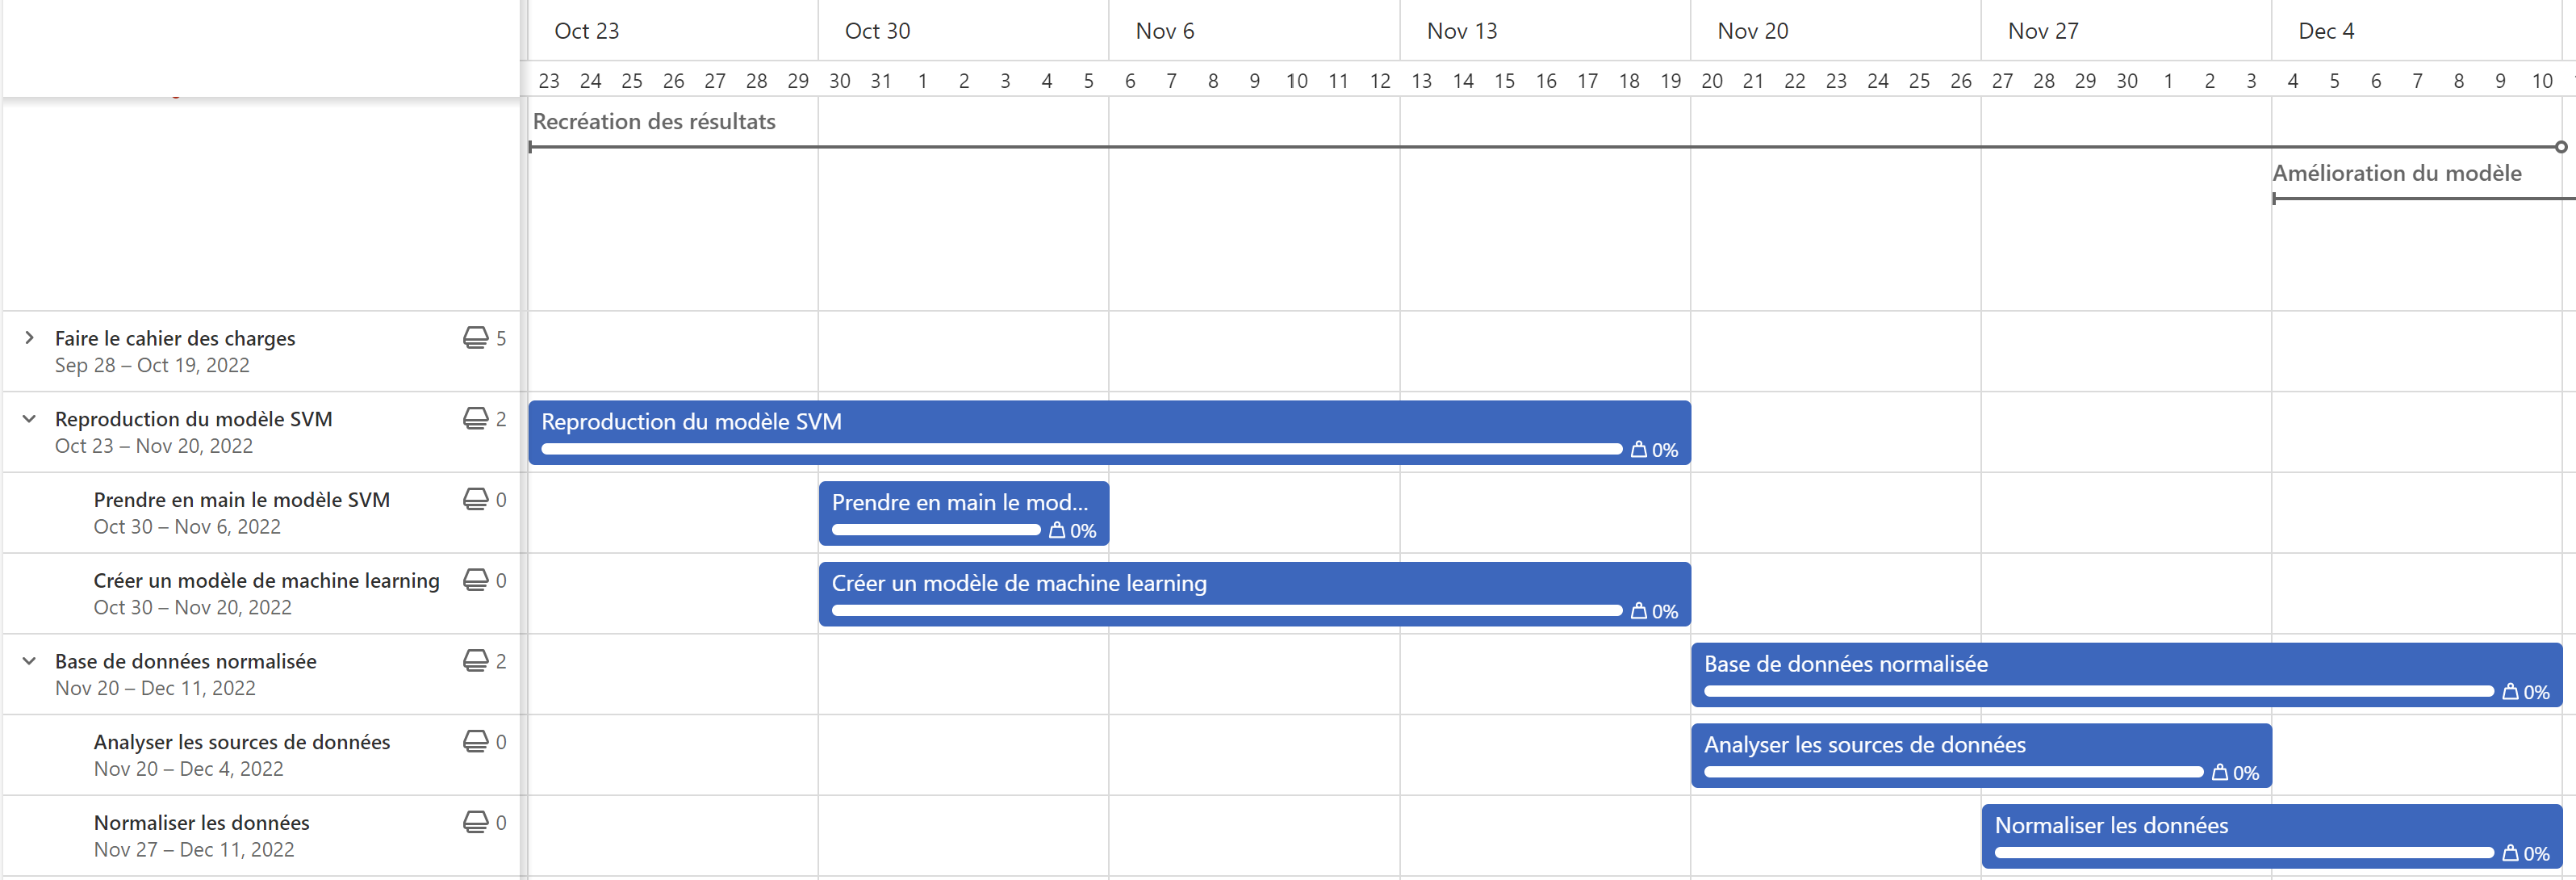
\includegraphics[width=14cm]{img/planning_1.png}
    \captionof{figure}{Planning de la recréation des résultats}
\end{center}

Ce premier planning représente la milestone qui correspond à la recréation des résultats. Il est composé de 2 épics principaux qui sont la base de données et le développement du premier modèle d'intelligence artificielle.

\begin{center}
    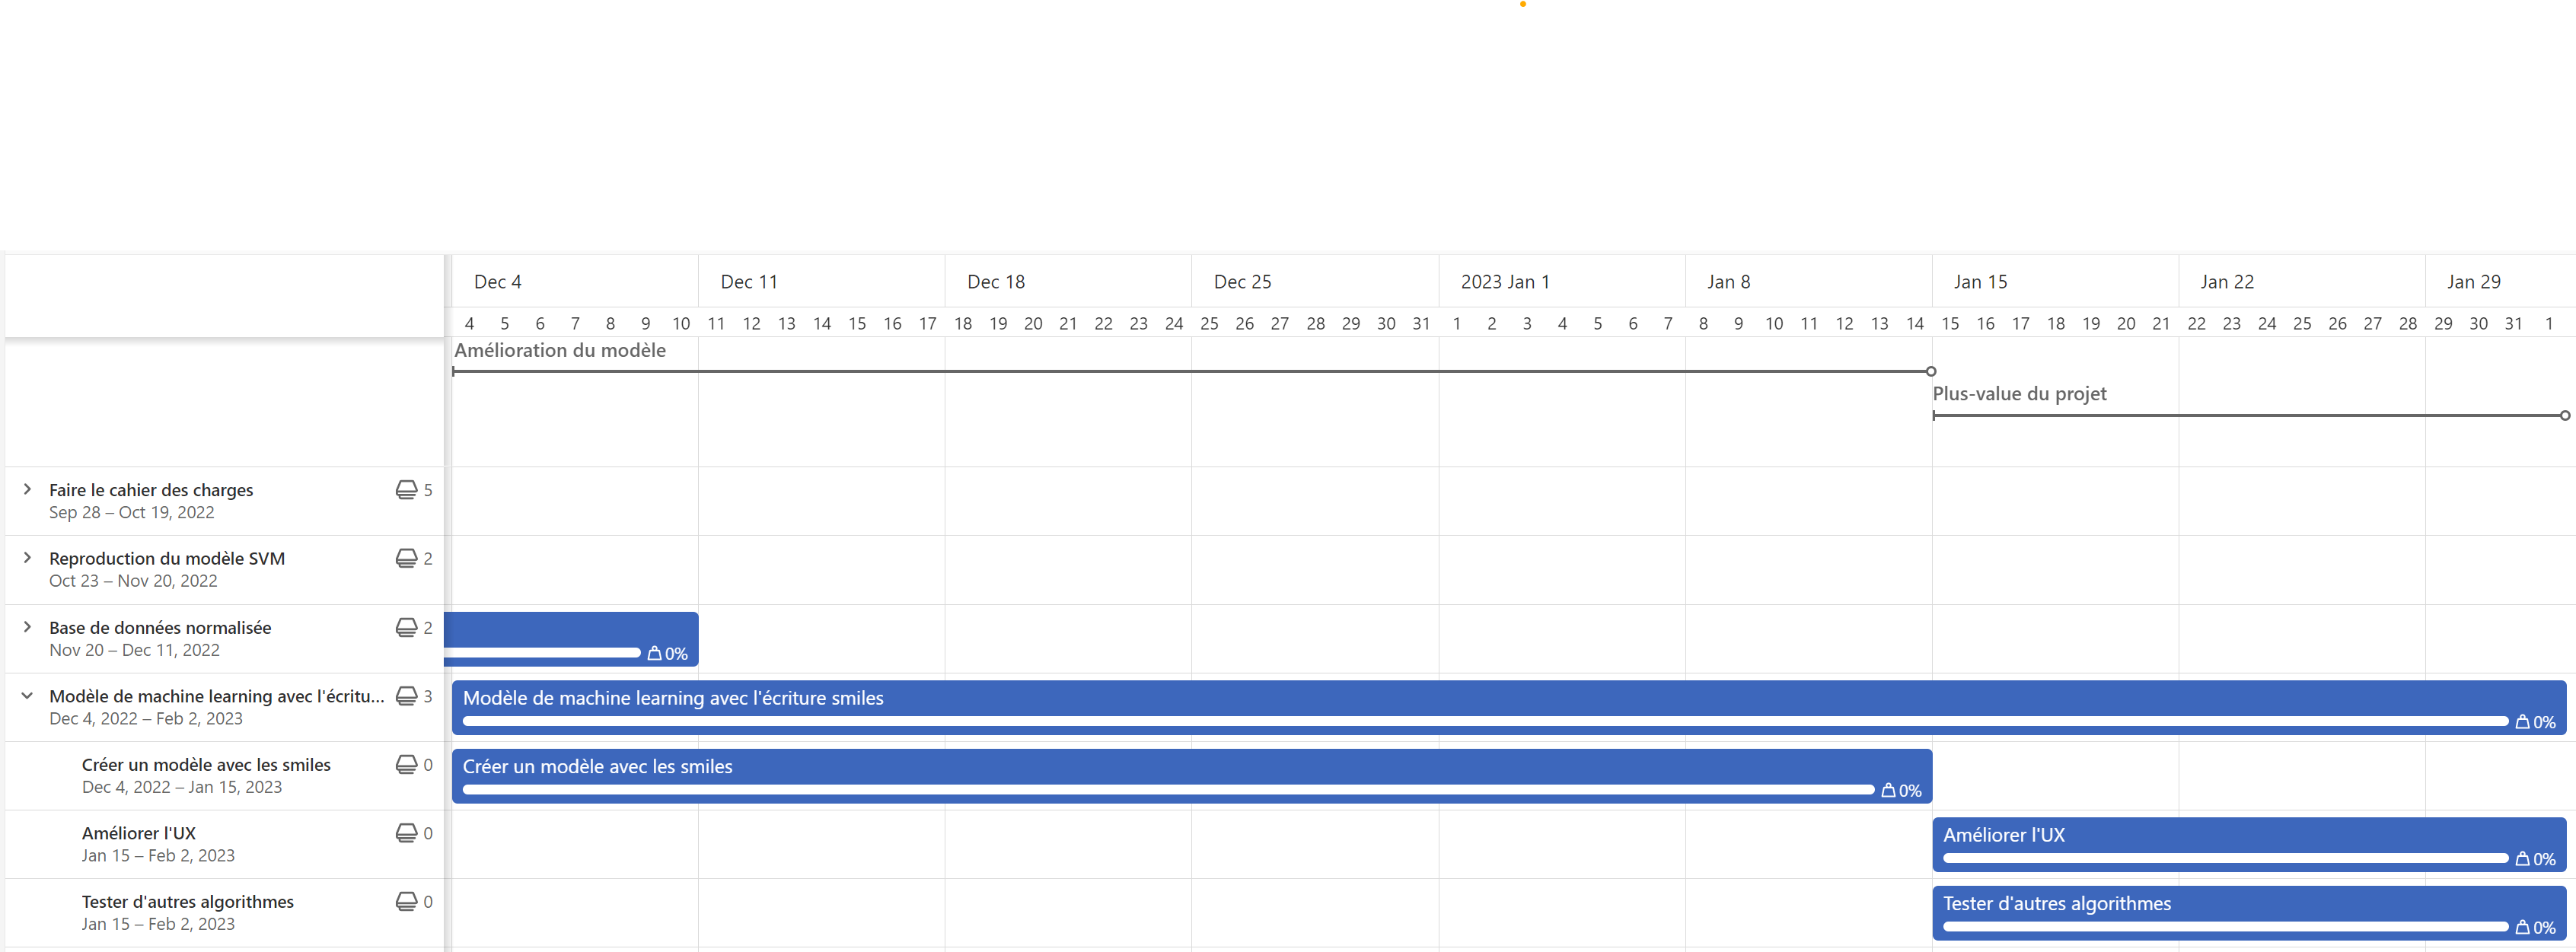
\includegraphics[width=14cm]{img/planning_2.png}
    \captionof{figure}{Planning de l'amélioration du modèle}
\end{center}

Cette deuxième partie de planing met en avant l'amélioration du modèle de machine learning à l'aide de l'écriture \acrshort{smiles}.
Elle est coupée par une milestone qui correspoond à la décision qui sera prise pour la finalisation du projet. En cas de résultats satisfaisants, nous nous concentrons sur les améliorations de l'expérience utilisateur avec une \acrshort{api}, une interface graphique ou autre solution.
Dans le cas contraire, nous pourrons essayer d'autres algorithmes afin d'améiorer les résultats de la prédiction.